\documentclass[11pt,a4paper]{article}

\usepackage[utf8]{inputenc}
\usepackage[T1]{fontenc}
\usepackage{lmodern}
\usepackage{amsmath,amssymb,amsthm,mathtools}
\usepackage{microtype}
\usepackage[colorlinks=true,citecolor=blue,linkcolor=blue,urlcolor=blue]{hyperref}
\usepackage{booktabs}
\usepackage{array}
\usepackage{longtable}
\usepackage{seqsplit}
\usepackage{enumitem}
\usepackage{tikz}
\usetikzlibrary{arrows.meta,positioning,calc}
\usepackage{listings}
\usepackage{xcolor}
\usepackage[margin=1in]{geometry}
\usepackage{cleveref}
\usepackage{needspace}
\usepackage[most]{tcolorbox}
\usepackage{expl3}
\usepackage{xparse}

\setlength{\hfuzz}{3pt}

\ExplSyntaxOn
\tl_new:N \l__ntl_leanref_tl
\NewDocumentCommand \leanref { m }
  {
    \tl_set:Nn \l__ntl_leanref_tl { #1 }
    \regex_replace_all:nnN { \c{_} } { \c{_} \c{allowbreak} } \l__ntl_leanref_tl
    \regex_replace_all:nnN { \. } { . \c{allowbreak} } \l__ntl_leanref_tl
    \regex_replace_all:nnN { ([a-z])([A-Z]) } { \1 \c{allowbreak} \2 } \l__ntl_leanref_tl
    \regex_replace_all:nnN { ([0-9])([A-Z]) } { \1 \c{allowbreak} \2 } \l__ntl_leanref_tl
    \texttt{\small \tl_use:N \l__ntl_leanref_tl }
  }
\ExplSyntaxOff

\newenvironment{keybox}[1]{%
  \Needspace*{8\baselineskip}%
  \begin{tcolorbox}[
    enhanced, breakable=false,
    colback=blue!5, colframe=blue!45!black, coltitle=black,
    colbacktitle=blue!14, boxrule=0.85pt, arc=2.5pt,
    left=9pt, right=9pt, top=6pt, bottom=6pt,
    titlerule=0.55pt, fonttitle=\bfseries, title={#1},
    before upper=\raggedright,
    before skip=0.9\baselineskip, after skip=0.9\baselineskip
  ]%
}{%
  \end{tcolorbox}%
}

% Compact, skimmable proof / witness notes (lighter than keybox).
\newenvironment{proofsketch}{%
  \par\smallskip
  \begin{tcolorbox}[
    enhanced, breakable,
    colback=blue!4, colframe=blue!28, boxrule=0.55pt, arc=2pt,
    left=8pt, right=8pt, top=5pt, bottom=5pt,
    before skip=0.35\baselineskip, after skip=0.45\baselineskip,
    fontupper=\small
  ]
  \noindent\textbf{Proof sketch.}\quad\ignorespaces
}{\end{tcolorbox}}

\newenvironment{witnessmeta}{%
  \par\smallskip
  \begin{tcolorbox}[
    enhanced, breakable=false,
    colback=gray!7, colframe=gray!55, boxrule=0.45pt, arc=2pt,
    left=8pt, right=8pt, top=5pt, bottom=5pt,
    before skip=0.25\baselineskip, after skip=0.4\baselineskip,
    fontupper=\small
  ]
}{\end{tcolorbox}}

\definecolor{leanblue}{RGB}{0,0,180}
\definecolor{leangreen}{RGB}{0,128,0}
\definecolor{leangray}{RGB}{128,128,128}
\lstdefinelanguage{Lean4}{
  keywords={theorem,def,lemma,example,structure,namespace,end,import,
            open,section,variable,where,by,exact,have,let,show,calc,
            intro,apply,rw,simp,omega,ring,linarith,native_decide,
            unfold,obtain,rcases,use,constructor,refine,induction,with},
  keywordstyle=\color{leanblue}\bfseries,
  commentstyle=\color{leangray}\itshape,
  stringstyle=\color{leangreen},
  morecomment=[l]{--},
  morecomment=[n]{/-}{-/},
  sensitive=true,
  basicstyle=\ttfamily\small,
  breaklines=true,
  columns=flexible,
  literate={→}{$\to$}1 {←}{$\leftarrow$}1 {∀}{$\forall$}1 {∃}{$\exists$}1
           {∧}{$\wedge$}1 {∨}{$\vee$}1 {¬}{$\neg$}1 {≤}{$\le$}1
           {≥}{$\ge$}1 {≠}{$\ne$}1 {∈}{$\in$}1 {ℕ}{$\mathbb{N}$}1
}
\lstset{language=Lean4}

\newtheorem{theorem}{Theorem}[section]
\newtheorem{lemma}[theorem]{Lemma}
\newtheorem{proposition}[theorem]{Proposition}
\newtheorem{corollary}[theorem]{Corollary}
\theoremstyle{definition}
\newtheorem{definition}[theorem]{Definition}
\newtheorem{remark}[theorem]{Remark}

\newcommand{\lean}{\textsc{Lean}\,4}
\newcommand{\NT}{\mathsf{NT}}
\newcommand{\Gen}{\mathsf{Gen}}
\newcommand{\Reg}{\mathsf{Reg}}
\newcommand{\Phase}{\mathsf{Phase}}
\newcommand{\Expl}{\mathsf{Expl}}
\newcommand{\Adeq}{\mathsf{Adeq}}
\newcommand{\Reduce}{\mathsf{Reduce}}
\newcommand{\ConservativeOver}{\mathsf{ConservativeOver}}
\newcommand{\GeneratedBy}{\mathsf{GeneratedBy}}
\newcommand{\ParadigmShift}{\mathsf{ParadigmShift}}
\newcommand{\ProvesAt}{\mathsf{ProvesAt}}
\newcommand{\HoldsAt}{\mathsf{HoldsAt}}
\newcommand{\ExpressibleAt}{\mathsf{ExpressibleAt}}
\newcommand{\FutureDefeat}{\mathsf{FutureDefeat}}
\newcommand{\Terminal}{\mathsf{Terminal}}
\newcommand{\Structural}{\mathsf{Structural}}
\newcommand{\Admissible}{\mathsf{Adm}}
% Breakable typewriter tokens (e.g.\ long identifiers in narrow table columns)
\newcommand{\ttwrap}[1]{{\ttfamily\seqsplit{#1}}}

\title{\textbf{Self-Transcending Generators:}\\
Fixed Causal Laws Without Final Explanatory Closure}
\author{Nova Spivack}
\date{}

\begin{document}
\maketitle

\begin{abstract}
\noindent
A hidden creed governs much contemporary thought: if a phenomenon is generated by fixed fundamental laws, then there must exist a fixed final explanatory language in which everything important about it can be said. The creed is false in a sharply formal sense. A finitely specified lawful generator can generate the whole future of its phases and still admit no fixed admissible explanatory closure.

\smallskip
\noindent
The theory ascends four linked summits. First, fixed lawful generation without fixed final explanation: every phase lies in the generator's causal trace, yet every admissible explanatory interface fails somewhere on the tower. Second, infinite conservative paradigm towers: explanatory succession can preserve prior adequacy while still forcing genuinely new structure. Third, upward explanatory necessity: later generated regimes can become necessary to express or prove structural truths about the generator itself. Fourth, generalized transfer: the phenomenon is not an artifact of one witness, one carrier, or one encoding, but survives transport across a nontrivial admissible class.

\smallskip
\noindent
Philosophically, this yields a third option. Everything in the tower remains generated from below under fixed law, yet explanation need not bottom out where causation bottoms out. The formal package does not entail indeterminism, backward causation, a universal diagonal over all raw interfaces, or universal infinite paradigm chains for every regime family. It establishes, instead, the existence, rigor, and transfer of lawful self-transcending structures: generated from below, but not finitely closed from below.

\smallskip
\noindent
\textbf{Strengthening layer (natural class).} Beyond the original generalized-crown transfer, the companion library also packages output-enum strict ascent across \emph{every} aligned natural admissible instance (not only the historic $\texttt{Bool}{\times}\mathbb{N}$ carriers), together with weak naturality hypotheses, organization-scale obstructions under explicit natural predicates, and disjunctive anti-closure packaging on natural numeric systems. Quantifiers remain honest: nothing in that layer claims a universal over all deterministic generators without the predicates stated in the formal statements.
\end{abstract}

\tableofcontents

\section{Introduction}

\begin{quote}
If a phenomenon is generated by fixed fundamental laws, then in principle there exists a fixed final explanatory language in which everything important about that phenomenon can be said.
\end{quote}

That creed is one of the deepest unexamined assumptions in modern thought. The theory developed here overturns it.

The thesis is not that laws fail, that causation fails, or that later phases are ungenerated. It is sharper: a system can be causally complete without being explanatorily final. A fixed law can produce every phase that appears and still defeat every would-be final reducer drawn from a nontrivial admissible class.

\begin{figure}[htbp]
  \centering
  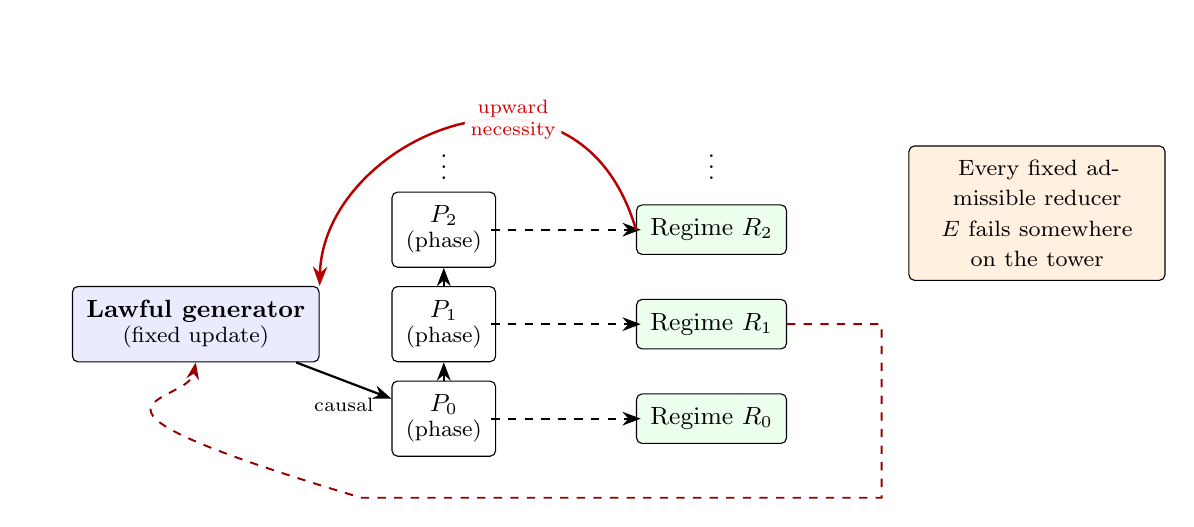
\begin{tikzpicture}[
    font=\small,
    grnode/.style={draw, rounded corners=2pt, inner sep=5pt, align=center},
    ca/.style={-Stealth, thick},
    ex/.style={-Stealth, thick, dashed},
    up/.style={-Stealth, line width=0.88pt, red!72!black}
  ]
    \node[grnode, fill=blue!8, minimum width=2.45cm] (G) at (0,2.35)
      {\textbf{Lawful generator}\\[-2pt]\footnotesize (fixed update)};
    \node[grnode] (P0) at (3.15,1.15) {$P_0$\\[-2pt]\footnotesize (phase)};
    \node[grnode] (P1) at (3.15,2.35) {$P_1$\\[-2pt]\footnotesize (phase)};
    \node[grnode] (P2) at (3.15,3.55) {$P_2$\\[-2pt]\footnotesize (phase)};
    \node at (3.15,4.45) {$\vdots$};
    \node[grnode, fill=green!7] (R0) at (6.55,1.15) {Regime $R_0$};
    \node[grnode, fill=green!7] (R1) at (6.55,2.35) {Regime $R_1$};
    \node[grnode, fill=green!7] (R2) at (6.55,3.55) {Regime $R_2$};
    \node at (6.55,4.45) {$\vdots$};

    \draw[ca] (G) -- (P0)
      node[pos=0.5, below=5pt, font=\scriptsize, inner sep=1pt] {causal};
    \draw[ca] (P0) -- (P1);
    \draw[ca] (P1) -- (P2);

    \draw[ex] ($(P0.east)-(0.06,0)$) -- ($(R0.west)+(0.06,0)$);
    \draw[ex] ($(P1.east)-(0.06,0)$) -- ($(R1.west)+(0.06,0)$);
    \draw[ex] ($(P2.east)-(0.06,0)$) -- ($(R2.west)+(0.06,0)$);

    \node[grnode, fill=orange!12, text width=2.9cm, anchor=north west] (Efail) at (9.05,4.62)
      {\footnotesize Every fixed admissible reducer $E$ fails somewhere on the tower};

    % Upward necessity: arc stays in a high band (well above $P_2$ and $\vdots$)
    \draw[up]
      (R2.west)
      .. controls ($(R2.west)+(-0.75,2.55)$) and ($(G.north east)+(0.05,1.9)$) .. (G.north east)
      node[pos=0.37, font=\scriptsize, text=red!85!black, align=center, inner sep=2pt,
           fill=white, fill opacity=0.94, text opacity=1, rounded corners=1.5pt] {upward\\necessity};

    % Representative feedback: east of $R_1$, then \emph{past} $R_0$ on the far right, then down and under $P_0$
    \coordinate (r1Exit) at ($(R1.east)+(0.28,0)$);
    \coordinate (pitLow) at ($(P0.south)+(0,-0.52)$);
    \coordinate (genApproach) at ($(G.south)+(-0.1,-0.55)$);
    % Vertical lane cleared to the right of every regime box (same $x$ stack as $R_0$)
    \coordinate (feederEast) at ($(R0.east)+(1.2,0)$);
    \coordinate (feederTop) at (feederEast |- r1Exit);
    \coordinate (feederBot) at (feederEast |- pitLow);
    \draw[up, red!58!black, line width=0.7pt, dashed]
      (R1.east) -- (r1Exit) -- (feederTop) -- (feederBot)
      -- ($(pitLow)+(-1.05,0)$)
      .. controls ($(G.south west)+(-0.55,-0.45)$) and (genApproach) .. (G.south);

  \end{tikzpicture}
  \caption{Conceptual spine (not a module graph): lawful generation drives phases upward along causal order; explanatory regimes attach to phases; every fixed admissible explanatory reducer fails somewhere; upward explanatory necessity feeds back toward structural truths of the generator. A further certification layer (weak naturality hypotheses, broad transfer across aligned \texttt{NaturalAdmissibleInstance} carriers, and packaged organization / anti-closure obstructions under explicit natural predicates) tightens the story against a narrowly ``engineered admissibility'' reply; see \Cref{sec:generalized-crown} and \Cref{tab:strengthened-lean}. Explanatory dependence need not mirror causal order.}
  \label{fig:conceptual-spine}
\end{figure}

What would be unsurprising is a world in which outputs merely outstrip a fixed vocabulary, observers run out of time, or simulation remains expensive. What the theorem package delivers is stronger: a single finitely specified generator can causally produce an infinite tower of phases and explanatory regimes such that no fixed admissible explanatory interface is final for that tower, and later generated regimes can become necessary for structural truths about the generator itself.

\begin{keybox}{The five central claims}
\textbf{1. Fixed law without fixed final explanation.} A single finitely specified generator can produce an infinite family of phases while no fixed admissible explanatory regime uniformly captures them all.

\medskip
\textbf{2. Infinite conservative paradigm towers.} Later regimes can preserve prior phase adequacy and still force genuinely new explanatory structure.

\medskip
\textbf{3. Upward explanatory necessity.} Later generated regimes can become necessary to express or prove structural truths about the generator's own long-run behavior.

\medskip
\textbf{4. Lawful self-transcendence with generalized transfer.} The architecture is neither anti-determinist nor merely rhetorical `emergence'; the flagship pattern survives transport beyond a single distinguished witness model.

\medskip
\textbf{5. Naturality-aware strengthening (honest quantifiers).} Under explicit weak naturality and \texttt{NaturalAdmissibleInstance} hypotheses, the output-enum strict-gap pattern transports to every aligned carrier in that class (not only the historic $\texttt{Bool}{\times}\mathbb{N}$ staging ground); bounded natural organization cannot certify totality of the standard future; and packaged anti-closure statements hold on \texttt{NaturalNumericSystem}---without claiming universality over all deterministic systems or all raw admissible interfaces (\Cref{sec:generalized-crown}, \Cref{tab:strengthened-lean}).
\end{keybox}

Three tasks structure the argument: introduce the self-transcending generator as a new species of mathematical object; state the theorem family that makes lawful non-finality unavoidable in the formal setting (including the naturality-aware strengthening layer where applicable); and draw the philosophical thesis that explanation need not bottom out where causal generation bottoms out.

\medskip
\noindent
The roadmap is as follows. \Cref{sec:nottrivial} explains what would be trivial and why this is not that. \Cref{sec:causal-vs-explanatory} separates causal generation from explanatory reducibility and fixes the informal schema. \Cref{sec:self-transcending} presents the flagship object. \Cref{sec:paradigm-shift} gives paradigm shift structural weight. \Cref{sec:first-summit} and \Cref{sec:no-final-internal} are the first two summits. \Cref{sec:generalized-crown} foregrounds the generalized final crown package, class transfer, and the naturality-aware strengthening layer (including \Cref{tab:strengthened-lean}). \Cref{sec:witnesses-proofs} collects the witness systems, proof sketches, and \lean{} theorem anchors. \Cref{sec:upward-necessity} is the crown summit. \Cref{sec:order-divergence} and \Cref{sec:retro} develop explanatory versus causal order and retrospective intelligibility. \Cref{sec:comparisons} states sharp non-equivalences and contrasts with chaos, computational irreducibility, and emergence rhetoric. \Cref{sec:philosophical} closes the philosophical arc. \Cref{sec:boundaries} states exactly what is and is not proved. \Cref{fig:conceptual-spine} orients the reader visually.

\section{What would be trivial, and why this is not that}\label{sec:nottrivial}

The theory would be uninteresting if it merely proved one of the following:

\begin{itemize}[leftmargin=2em]
\item a fixed language eventually fails on sufficiently rich outputs;
\item complexity can outrun a bounded observer;
\item prediction can become hard or impossible;
\item a process can have infinitely many outputs;
\item one can always invent richer descriptive vocabulary after the fact.
\end{itemize}

Each of these is real, but none is enough. None produces the kind of inversion this project seeks.

The actual target is a much stronger conjunction. We want a finitely specified generator $G$ and a family of phases and regimes $(P_n,R_n)$ such that

\begin{enumerate}[leftmargin=2em]
\item every $P_n$ is generated by $G$;
\item each $R_n$ adequately explains $P_n$ in the formal sense of the theory;
\item each successor transition is conservative over prior history and irreducible to the prior regime;
\item every fixed admissible explanatory interface fails somewhere on the tower;
\item later regimes can become necessary for structural truths about the generator itself.
\end{enumerate}

It is not a theorem of mere output richness, brute infinitude, or observational unpredictability alone. It is a theorem of \emph{non-final explanation under fixed law}.

That is why the project must be read as a theory of lawful self-transcendence. The center of gravity is not ``more happens than we can compress cheaply.'' It is: ``fixed lawful generation does not guarantee fixed final explanation.'' A single fixed generator can causally produce an infinite tower of phases and regimes such that none are uniformly collapsible into a fixed admissible interface, and later regimes can become necessary for truths about the generator itself.

\section{Causal generation versus explanatory reducibility}\label{sec:causal-vs-explanatory}

The core distinction is between two relations:

\begin{itemize}[leftmargin=2em]
\item \textbf{Causal generation:} the system produces a phase, state, or phenomenon as part of its lawful trace.
\item \textbf{Explanatory reducibility:} a fixed admissible regime suffices to preserve the relevant structural distinctions, adequacy conditions, and invariant content.
\end{itemize}

These are not the same relation---and treating them as identical is exactly how the hidden creed smuggles in final closure.

To say that a phase is generated is a constructive or causal claim. To say that it is reducible to a fixed admissible regime is stronger: it requires structural adequacy without loss of the certified distinctions the theory cares about.

\begin{definition}[Informal self-transcendence schema]
A generator $G$ is self-transcending, in the core sense of the present framework, if there exists a sequence $(P_n,R_n)_{n\in\mathbb{N}}$ such that:
\[
\forall n,\; \GeneratedBy(G,P_n),
\quad
\forall n,\; \Adeq(R_n,P_n),
\quad
\forall n,\; \ParadigmShift(R_n,R_{n+1};P_{\le n}),
\]
and
\[
\forall E \in \Admissible,\; \exists n,\; \neg \Expl(E,G,P_n,R_n).
\]
\end{definition}

The force of this definition is easy to miss. The theorem is not merely that later phases need later words. It is that \emph{every fixed admissible explanatory reducer fails somewhere}. This is the structural anti-closure statement.

\begin{quote}
\textbf{Causal sufficiency does not imply explanatory closure.}
\end{quote}

That sentence is the lens through which everything below should be read.

\section{Self-transcending generators: a new species of object}\label{sec:self-transcending}

The self-transcending generator is not a rhetorical flourish; it is the field-defining object of the theory. If such objects exist cleanly under honest admissibility hypotheses, the program is worth doing---not as cataloguing a formal artifact, but because they carve out a new structural possibility in the conceptual space of law, explanation, and reduction.

\medskip
\noindent
\textbf{Why this is not ``a complicated dynamical system.''}
A generator with intricate outputs, a hard-to-predict future, or a long run of surprising behavior may still admit a fixed explanatory regime that is final relative to the admissible class. The self-transcending generator is characterized by the \emph{failure} of that finitude: the causal trace is fully owned by one fixed law, while explanatory closure is systematically defeated for every admissible reducer at some height on the tower. Complexity alone does not imply that joint profile.

\medskip
\noindent
\textbf{Why the object is field-defining.}
Much of science and philosophy silently assumes that tightening law and tightening explanation march together. The self-transcending generator is the minimal schematic shape of their divergence: one fixed engine; inexhaustible stratification of adequate regimes; conservative, irreducible transitions; universal failure of any fixed final interface; and (at the crown) upward necessity for truths about the source itself. Theorems about this shape are not marginal remarks about pathological examples; they are theorems about what \emph{lawful explanation} can and cannot promise.

\medskip
\noindent
\textbf{Why existence is philosophically radical.}
If even one such generator fits the formal package, the hidden creed cannot be treated as analytic. It becomes an empirical-conceptual hostage: perhaps nature never realizes the package, but \emph{in principle} fixed law without final explanation is coherent, structured, and provable. That shifts the default: final closure must be earned, not assumed from the fact of generation.

\begin{enumerate}[leftmargin=2em]
\item the phases are generated by the same fixed law;
\item the corresponding regimes are genuinely adequate for the phases they explain;
\item the transitions between regimes are conservative over prior history;
\item those transitions are structurally irreducible;
\item no fixed admissible explanatory interface is final for the whole tower.
\end{enumerate}

\begin{quote}
\textbf{A system can generate what it cannot finitely finish explaining.}
\end{quote}

That slogan marks the place where ordinary complexity talk ends and a new mathematical possibility begins: not merely many states, but lawful generation without fixed explanatory closure.

What makes the self-transcending generator a new mathematical object is therefore not that it has many states, nor that it surprises bounded observers, but that it occupies a new structural category: exact generation without final explanatory closure. If such objects exist, then explanatory non-finality is not a symptom of epistemic weakness alone; it is a lawful structural possibility.

\section{Paradigm shift as a formal object}\label{sec:paradigm-shift}

One of the deepest aims is to rescue ``paradigm shift'' from sociological fog and give it a structural backbone. The target is not arbitrary language change, nor a destructive rewrite of the past, nor metaphorical ``revolution.'' It is a disciplined pattern: non-destructive transitions that nonetheless force genuine novelty in what can be explained and certified.

\subsection{Conservative extension}

The successor regime $R_{n+1}$ must respect what $R_n$ already secured on the available history $H_n$. Conservativity is the guarantee that the revolution is not vandalism: prior adequacy on certified past structure is preserved when passing upward. Without that constraint, the notion collapses into mere replacement; with it, novelty must squeeze through a narrow gate---it must arrive \emph{despite} honest retention of what came before.

\subsection{Irreducibility}

At the same time, $R_{n+1}$ must not be a notational variant of $R_n$ for the new work at stake. There must be generated structure that $R_n$ cannot adequately treat while $R_{n+1}$ can. Irreducibility is the mathematical content of ``genuinely new explanatory structure'': not convenience, but loss of collapse into the prior admissible basis for the relevant claims.

\subsection{Why this is paradigm shift, not metaphor}

This is why the theorem package around infinite conservative paradigm towers is not a decorative extension of the theory but one of its deepest results. It shows that explanatory revolution need not be either destructive or merely sociological. It can be historically conservative, mathematically necessary, and still irreducible to any fixed earlier admissible regime. In that sense, paradigm shift becomes a structural theorem rather than a metaphor.

\medskip
\noindent
Formally, a paradigm shift here is a transition from $R_n$ to $R_{n+1}$ over $H_n$ such that:
\begin{enumerate}[leftmargin=2em]
\item $R_n < R_{n+1}$;
\item $\ConservativeOver(H_n,R_n,R_{n+1})$;
\item there exists a new generated phase $P_{n+1}$ with
\[
\neg \Adeq(R_n,P_{n+1}) \wedge \Adeq(R_{n+1},P_{n+1});
\]
\item the new regime is not reducible to the old one with respect to the relevant structural content.
\end{enumerate}

\section{The first summit: fixed generation without fixed final explanation}\label{sec:first-summit}

The first summit proves that the explanatory tower is never uniformly absorbed by a fixed admissible interface.

\[
\exists G\,\exists (P_n,R_n)_{n\in\mathbb{N}}\,
\Bigl[
\forall n\,\GeneratedBy(G,P_n)
\wedge
\forall E\in\Admissible\,\exists n\,\neg \Expl(E,G,P_n,R_n)
\Bigr].
\]

The system remains perfectly lawful; the law generates the whole trace. What fails is final explanation---not because forecast is hard within a fixed architecture, but because \emph{no} architecture of the admissible kind is final across the tower.

This is the first point at which the theory reveals itself as a theory of non-final explanation rather than merely a theory of complicated systems. The point is not that some interface happens to fail. It is that every fixed admissible interface fails somewhere. That is the first true rupture with the hidden creed.

\begin{keybox}{The first summit}
\textbf{A fixed finitely specified generator can produce every relevant phase causally, and yet no fixed admissible explanatory regime is final for the whole generated future.}
\end{keybox}

\section{The second summit: no final internal theory}\label{sec:no-final-internal}

The no-final-internal-theory form is stronger than ``some representation wears out.''
\begin{quote}
There is no admissible internal theory of the relevant type that is final for the generated future.
\end{quote}

Finality itself becomes impossible in the specified class---not a local glitch but explanatory anti-closure:
\[
\text{fixed law} \;\not\Rightarrow\; \text{fixed final internal theory}.
\]

This is already a very strong claim. It is still not the crown.

The significance of this theorem is not merely technical. It blocks a familiar escape route: the thought that perhaps there is still, somewhere in the architecture, a final internal standpoint from which the whole future explanatory story can be closed. In the relevant formal setting, there is not. The failure is not local but architectural.

\section{The generalized final crown package}\label{sec:generalized-crown}

The flagship claim of the companion certification is not a scattered list of curiosities. It is the \textbf{generalized final crown}: a single articulated package in which the philosophical inversion is backed by a coordinated family of results. The generalized final crown package is the point at which the central philosophical thesis becomes fully theoremic. The earlier summit stack already establishes non-finality and ascent. The generalized crown shows that this is not a quirk of one witness, one encoding, or one carrier, but a transferable structural phenomenon. Read as one backbone rather than as isolated peaks, the package includes, in order of conceptual dependence:

\begin{enumerate}[leftmargin=2em]
\item \textbf{Generalized iterated structural ascent.} Strict proof-theoretic ascent for structurally certified sentences along the packaged regimes.
\item \textbf{Generalized no fixed structural stratum.} No fixed structural stratum of the relevant formal class is final for the generated future---an anti-closure claim stronger than a one-step gap.
\item \textbf{Generalized future defeat of terminality.} Would-be terminality-style universal bounds are defeated in a future-directed, packaged sense for the canonical tower.
\item \textbf{Generalized generator-truth family.} Ascent is tied to truths about the generator itself, not to arbitrary propositional noise.
\item \textbf{Generalized class transfer.} The phenomenon is realized not only in one witness but across aligned carriers in a nontrivial admissible class.
\item \textbf{Generalized non-single-model artifact.} The gap pattern is certified \emph{not} to be merely an artifact of one model, one encoding, or one carrier.
\end{enumerate}

Taken together, these clauses do not merely strengthen the earlier crown. They change its status. What was first proved as a dramatic existence result is now shown to persist across a disciplined admissible class. That is what turns the phenomenon from a striking witness into the beginning of a theory.

The crown phenomenon would be dramatically weaker if it held only in one hand-picked model. Transfer is what blocks the cheap escape: ``this is a trick of the presentation.'' When the same structural failure class recurs under disciplined transport while traces remain genuinely distinct in the relevant sense, the philosophical reading strengthens: one is not watching a coding accident but a reproducible pattern of lawful non-finality.

\medskip
\noindent
The $\texttt{Bool}{\times}\mathbb{N}$ twin construction remains the canonical \emph{existential} staging ground for \textbf{class transfer} in the summit package, because it supplies two concrete aligned generators with trace-level mismatch. The strengthening layer recorded in \Cref{tab:strengthened-lean} then pushes the \emph{same} output-enum witness \texttt{ProvesAtCarrier} gap to \textbf{every} stage and every \texttt{NaturalAdmissibleInstance} (including $\mathbb{N}$-observation carriers), and packages further organization-scale and anti-closure consequences under predicates named in the formal artifact.

\begin{remark}[Lean packaging of the six crown clauses]
Each clause above is a named theorem in the generalized final crown package namespace. Iterated structural ascent: \leanref{NoveltyTheory.Summits.GeneralizedFinalCrownPackage.generalized\_final\_crown\_iterated\_structural\_ascent}. No fixed structural stratum (for every bound $B$): \leanref{NoveltyTheory.Summits.GeneralizedFinalCrownPackage.generalized\_final\_crown\_no\_fixed\_structural\_stratum}. Future defeat of terminality: \leanref{NoveltyTheory.Summits.GeneralizedFinalCrownPackage.generalized\_final\_crown\_future\_defeat\_of\_terminality}. Generator-truth family paired with ascent: \leanref{NoveltyTheory.Summits.GeneralizedFinalCrownPackage.generalized\_final\_crown\_generator\_truth\_family}. Class transfer: \leanref{NoveltyTheory.Summits.GeneralizedFinalCrownPackage.generalized\_final\_crown\_class\_transfer}. Non-single-model artifact: \leanref{NoveltyTheory.Summits.GeneralizedFinalCrownPackage.generalized\_final\_crown\_not\_model\_artifact}.
\end{remark}

\begin{remark}[Naturality, broader transfer, and inevitability packaging]
To address the ``specially engineered admissibility'' objection without pretending to universalize over all raw interfaces, the library adds: \textbf{(i)} weak naturality / adequacy infrastructure (\leanref{NoveltyTheory.Foundation.NaturalityFacts.naturality\_adequacy\_transport}); \textbf{(ii)} broad carrier transfer for every \texttt{NaturalAdmissibleInstance} via \leanref{NoveltyTheory.Ridge.BroadTransfer.naturalClass\_preserves\_structural\_ascent} and the packaged \leanref{NoveltyTheory.Ridge.BroadTransfer.broad\_transfer\_of\_generalized\_crown}; \textbf{(iii)} bounded-organization obstructions under \texttt{NaturalBoundedOrganization} (\leanref{NoveltyTheory.Ridge.UnboundedOrganization.natural\_no\_final\_organization\_theorem}); and \textbf{(iv)} disjunctive anti-closure on \texttt{NaturalNumericSystem} (\leanref{NoveltyTheory.Ridge.NaturalAntiClosure.natural\_anti\_closure\_theorem}). Headline prose should cite these identifiers only when the quantifiers match the formal statements.
\end{remark}


\medskip
\noindent
For witness systems, proof sketches, and \lean{} theorem anchors keyed to the crown package above, see \Cref{sec:witnesses-proofs}.

\section{The crown summit: upward explanatory necessity}\label{sec:upward-necessity}

\textit{This section is the central summit of the argument.}

If there is a single theoremic-philosophical center of gravity, it is here. The earlier summits establish that fixed lawful generation need not yield fixed final explanation. The present summit goes further: it shows that later generated regimes can become necessary, not merely for later phases, but for structural truths about the generator itself. \textbf{This is the inversion theorem.}

The prior summits establish non-finality: no fixed admissible reducer closes the tower; no final internal theory of the relevant type settles the future story. What follows is the deeper inversion. Later generated explanatory regimes can become \emph{necessary} for structural truths about the generator itself. The causal order remains unchanged; what changes is explanatory dependence.

\medskip
\noindent
\textbf{Why it sounds contradictory.}
If the generator is the source of everything downstream, it is tempting to treat everything ``real'' about the process as already implicit in the source description. On that hearing, the idea that \emph{later} strata are indispensable for understanding the \emph{earlier source} feels like logical nonsense---as if the effect somehow authored the cause. That hearing conflates generation with explanation.

\medskip
\noindent
\textbf{Why it is not contradictory once the relations are separated.}
Generation answers: what states arise, in what order, under which fixed update? Explanation answers: which admissible regime is adequate for which structural truths, and what can be proved or expressed at which depth? Those are different questions. Nothing in the forward causal order is reversed when a later regime is required to \emph{state or prove} what an earlier regime could not. The source still generates the whole trace; the derivative layers remain causally downstream; what changes is where certain truths become visible, expressible, or provable.

\medskip
\noindent
\textbf{Why this flips reductionism rather than merely limiting it.}
A modest limitation story says: ``we lack a single brilliant final theory because we are finite.'' The crown says more. It says the hierarchy of intelligibility need not admit a final admissible stratum \emph{even in principle} relative to the class, and that later strata can be \emph{unavoidable} for truths about the source. That is not a gap in our patience; it is a structural feature of the explanatory relation under lawful generation.

\medskip
The usual picture runs like this:
\begin{enumerate}[leftmargin=2em]
\item the generator is fundamental;
\item the generated layers are derivative;
\item therefore the generated layers cannot be strictly necessary for understanding the generator except as convenience.
\end{enumerate}

The crown says step (3) can fail.

\[
\exists G,\exists(R_n),\exists(\Phi_n)\;
\forall n,\;
\Phi_n \text{ is a structural truth about } G
\;\wedge\;
\ProvesAt(R_{n+1},\Phi_n)
\;\wedge\;
\neg \ProvesAt(R_n,\Phi_n).
\]

Read verbally, the theorem says: for each stage there is a structural truth about the generator that becomes provable only from a later regime. The generator remains the source of the whole tower, but the tower it generates becomes necessary for understanding the generator itself.

The claim is not about later outputs alone. It is about structural truths of the source process: the derivative becomes necessary for understanding the source.

In the certification, the schematic $\Phi_n$ can be taken concretely from the retro-structural family \texttt{histSeqUpto}\,$n$---a finite diagonal history of trace-equalities $(i,i)$ for $i<n+1$---which is \texttt{IsStructuralSentenceV2} and satisfies $\texttt{ProvesAt}\,(n{+}1)\,\Phi_n \land \neg\texttt{ProvesAt}\,n\,\Phi_n$ (\leanref{NoveltyTheory.Foundation.RetroStructuralTruthV2.histSeqUpto}, \leanref{NoveltyTheory.Ridge.RetroStructuralGap.histSeqUpto\_proves\_succ\_not\_at}). Generator-anchored sentences such as \texttt{traceEq}\,$n\,n$ supply the ``truth about the counter'' side of the package alongside that ascent (\leanref{NoveltyTheory.Summits.GeneralizedFinalCrownPackage.generalized\_final\_crown\_generator\_truth\_family}).

\begin{keybox}{The crown inversion}
\textbf{Later generated explanatory regimes can become necessary for structural truths about the generator itself.}
\end{keybox}

\section{Explanatory order and causal order}\label{sec:order-divergence}

This section does three jobs at once.

\medskip
\noindent
\textbf{(1) Formal separation.}
Causal order is the forward structure of lawful production:
\[
s_0 \mapsto s_1 \mapsto s_2 \mapsto \cdots
\]
Explanatory order tracks where structural truths become expressible, adequate, or provable within admissible regimes. The two orders can diverge: a fact can be causally ``early'' while remaining explanatorily ``late.''

\medskip
\noindent
\textbf{(2) No backward causation.}
Upward explanatory necessity does not mean later regimes pull levers in the past. Causal sufficiency of the generator and forward dynamics are untouched. The inversion concerns intelligibility and proof-theoretic access, not forces traveling up the time arrow.

\medskip
\noindent
\textbf{(3) Upward dependence without causal reversal.}
Explanatory dependence can run from higher strata back toward truths about the generator \emph{without} reversing causal priority. Think of it as a second coordinate system laid over the same lawful trajectory: the causal coordinate orders production; the explanatory coordinate orders what must be said to honor the structure. They need not coincide.

\begin{quote}
\textbf{Explanatory order need not mirror causal order.}
\end{quote}

This is the opening for a new conception of explanation. Causal order may still run downward or forward from a fixed source, while explanatory dependence climbs upward through generated strata that the source itself necessitates but does not finitely close. That is the formal core of lawful self-transcendence.

\section{Retroactive structural revelation}\label{sec:retro}

Later regimes need not merely forecast the next segment of trace. Once explanatory order splits from causal order, a sharper phenomenon appears: later regimes can \emph{disclose latent structure in earlier history}---truths about $P_{\le n}$ that were not expressible, provable, or structurally visible from $R_n$, yet become available from $R_m$ for $m>n$.

\[
\exists n<m,\exists\Psi\;
\Bigl[
R_m \vdash \Psi(P_{\le n})
\wedge
R_n \not\vdash \Psi(P_{\le n})
\Bigr].
\]

Retroactive structural revelation is therefore not an incidental byproduct of the theory. It is one of its deepest consequences. Explanation grows not only by extending into the future but by reorganizing the intelligibility of the past. Later regimes do not merely forecast what comes next; they can disclose what had already been there without yet being structurally sayable. The certified template sentences \texttt{histSeqUpto}\,$n$ are exactly of this ``initial segment made explicit'' form (\leanref{NoveltyTheory.Foundation.RetroStructuralTruthV2.histSeqUpto}, \leanref{NoveltyTheory.Ridge.RetroStructuralGap.histSeqUpto\_proves\_succ\_not\_at}).

\section{Why this is not chaos, not computational irreducibility, not emergence rhetoric, and not mere bookkeeping}\label{sec:comparisons}

\subsection{Four surgical non-equivalences}

The main comparisons are four distinct failures of identification:
\begin{itemize}[leftmargin=2em]
\item \textbf{Generation $\neq$ explanation.} Lawful production of a phase does not entail its explanatory reducibility to any fixed admissible regime.
\item \textbf{Simulation $\neq$ explanatory reduction.} Stepping the dynamics can outrun explanatory collapse: exact generation does not hand you final understanding in the packaged sense.
\item \textbf{Observational sameness $\neq$ explanatory sameness.} Matching coarse traces does not settle adequacy for structurally certified truths at issue in the theory.
\item \textbf{Complexity growth $\neq$ explanatory non-finality.} ``Getting richer'' in an informal sense does not by itself imply the systematic failure of every fixed final reducer in an admissible class.
\end{itemize}

\subsection{Chaos}

Chaos: sensitive dependence and unstable long-term prediction \emph{within} a fixed explanatory architecture. Novelty theory: that architecture of the admissible kind may not be final across the tower at all. Difficulty $\neq$ systematic non-finality.

\subsection{Not computational irreducibility}

Computational irreducibility concerns the absence of substantial shortcuts for computing later states of a process. The present theory concerns something stronger and different: the absence of fixed final explanatory closure even for a fully lawful generated trace. One may have exact generation, exact simulation, or observational agreement and still lack explanatory reduction in the relevant formal sense. The issue here is not merely that the future is costly to compute; it is that explanation itself need not close under a fixed admissible regime.

\subsection{Not generic emergence rhetoric}

The framework does not rest on loose ``emergence,'' ``levels,'' or ``useful descriptions.'' It rests on admissible reductions, adequacy, conservative shifts, generator-anchored truths, and proof-theoretic ascent---where later structure can be mathematically necessary and not uniformly collapsible to any fixed prior admissible stance.

\subsection{Not ``merely engineered'' admissibility}

A common informal reply is that the crown depends on \emph{specially chosen} admissibility or coding. Two distinctions block a quick dismissal. First, explicit \textbf{obstruction lemmas} rule out illegitimate universal diagonal maneuvers over raw interfaces: the trust boundary is written into the formal predicates, not hidden. Second, the \textbf{strengthening layer} (\Cref{sec:generalized-crown}, \Cref{tab:strengthened-lean}) separates \textbf{weak naturality / adequacy transport} from \textbf{existence of a crown package}, extends the output-enum \texttt{ProvesAtCarrier} gap across all aligned \texttt{NaturalAdmissibleInstance} carriers (not only $\texttt{Bool}{\times}\mathbb{N}$), and states organization / anti-closure consequences under \texttt{NaturalBoundedOrganization} and \texttt{NaturalNumericSystem}. None of this asserts a universal over all deterministic systems; it does narrow the honest scope of a ``we engineered the admissible class'' complaint to the actual quantifiers in those theorems.

\subsection{Why this is not just incompleteness in disguise}\label{sec:not-incompleteness}

The theory is incompleteness-adjacent in atmosphere, but it is not merely Gödel reheated. Its central object is not a single formal calculus outrun by truth in the abstract. Its central object is a generated tower of phases and explanatory regimes under a disciplined admissibility class, together with the failure of fixed final explanatory closure for that tower. The crown result is stronger still: later generated regimes can become necessary for structural truths about the generator itself. That is a theorem of explanatory non-finality under exact generation, not just a rephrasing of formal incompleteness.

\section{Why this is not just genotype/phenotype}

Genotype/phenotype is a one-step manifestation gap. This theory is an unbounded tower with conservative irreducible succession and upward necessity at the crown. The analogy can at best illuminate the foothills. It cannot capture the theoremic heart of the argument, which is a multi-stage, formally disciplined, upwardly necessary architecture of explanatory non-closure.

\section{Lawful self-transcendence as a third philosophical option}\label{sec:philosophical}

Naïve reductionism: everything generated from below, therefore finally explainable from below. Mystification: if not reducible, then outside law or science. The third option: \textbf{lawful self-transcending structure}---fully generated, fully lawful, not finitely explanation-closed, with possible upward necessity.

\medskip
\noindent
\textbf{Why the mathematics matters.}
The framework supplies a rigorous language for separating mere complexity, mere redescription, genuine structural novelty, true explanatory phase shifts, and the \emph{non-collapse} of explanation under exact generation. Without such distinctions, debates about reduction, emergence, and explanation talk past one another. The point is not only that some formal possibility exists; it is that one can \emph{name} and \emph{prove} a coherent profile of lawful non-finality strong enough to break the hidden creed without breaking naturalism.

If this framework is right, then the deepest lesson is not merely that the future may surprise us, nor that science may need new theories. It is that full lawfulness and full generative completeness do not force final explanatory closure. The space of lawful systems is wider than reductionism assumed. That is why lawful self-transcendence is not only a new mathematical object, but a new philosophical possibility.

\medskip
\noindent
The companion certification additionally isolates a \textbf{naturality-aware} layer: weak principles link adequacy across stages, structural sentence families are checked against those principles, and output-enum ascent is transported across the whole \texttt{NaturalAdmissibleInstance} class together with organization and anti-closure packaging on explicitly \emph{natural} predicates. Prose that cites that layer must track those predicates and avoid turning them into forbidden raw-universal headlines.

\section{What is formally proved, and what lies outside scope}\label{sec:boundaries}

The text proves a strong but sharply scoped claim. In the formal setting developed alongside it, there exist packaged lawful generators realizing iterated structural ascent, failure of fixed final admissible explanatory closure, future defeat of terminality in the packaged sense, generator-anchored truth families, class transfer across a nontrivial admissible class (with concrete $\texttt{Bool}{\times}\mathbb{N}$ witnesses), and non-single-model-artifact results.

In the same artifact, a further family of theorems (summarized in \Cref{tab:strengthened-lean}) states \textbf{broad transfer} of the output-enum carrier gap for all aligned \texttt{NaturalAdmissibleInstance} values, \textbf{bounded natural organization} obstructions on the standard future predicate, and \textbf{natural anti-closure} packaging on \texttt{NaturalNumericSystem}---each under the hypotheses named in the corresponding \lean{} declarations.

What the formal package does not entail is equally important. It does not imply that every deterministic system exhibits the crown phenomenon, that every conceivable explanatory notion fails globally, that every organization must be infinite, or that causation runs backward. It does not imply a universal diagonal over all raw admissible interfaces, nor an infinite paradigm tower for every singleton-within regime family. Those literal universal glosses are false under the formal predicates where explicit obstruction applies.

This boundary is not a retreat. It is the condition of the theory's strength. The scoped theorem family is already sufficient to establish the existence, structure, and transfer of lawful non-final explanation under fixed law, and the strengthening layer adds rigorously scoped claims against a narrow ``presentation trick'' dismissal.

\section{Conclusion}

The hidden creed with which the argument began can no longer be treated as self-evident. Fixed law does not imply fixed final explanation.

In the formal setting developed here, a single lawful generator can produce an infinite tower of phases and explanatory regimes while defeating every fixed admissible explanatory interface of the relevant class. The succession can be conservative without being reducible, historically preserving what came before while forcing genuinely new explanatory structure. And at the crown, later generated regimes can become necessary for structural truths about the generator itself.

That conjunction is the real result. It is stronger than complexity growth, stronger than mere unpredictability, stronger than loose emergence talk, and stronger than a one-step manifestation gap. It identifies a new structural possibility: exact generation without final explanatory closure.

The philosophical consequence is equally clear. Explanation need not bottom out where causation bottoms out. A system may be fully lawful and fully generative without being finitely explanation-closed.

If that possibility is genuinely formal, then a new mathematics begins here: not merely a mathematics of what fixed laws generate, but a mathematics of when fixed laws fail to be explanatorily final for what they themselves produce.

\medskip
\noindent
The strengthening certification extends this picture: once carrier alignment and natural admissibility are fixed as in the library, the same witness-level ascent is not hostage to a single encoding of observations, and additional organization / anti-closure consequences are available under the corresponding natural predicates (\Cref{tab:strengthened-lean}).

\appendix

\section{Witness systems, proof sketches, and \lean{} anchors}\label{sec:witnesses-proofs}

This appendix is organized in small, parallel blocks. Each block lists \textbf{what is being formalized}, the main \lean{} certificates, and---when helpful---an isolated \emph{proof sketch} box. Skim the gray \textbf{At a glance} tiles first; dive into the blue \textbf{Proof sketch} tiles only when needed.

\subsection{Generative systems and the canonical counter}

\begin{witnessmeta}
\textbf{At a glance.}\quad A discrete-time deterministic generator emits an infinite observable trace. The default dynamical witness is a bare counter on $\mathbb{N}$ whose trace is the identity.
\end{witnessmeta}

\begin{itemize}[leftmargin=1.6em, itemsep=0.35em]
\item \textbf{Formal generator.} State $S$, observations $X$, parameters $(s_0,\tau,\mathrm{out})$, trace $\mathrm{trace}_G(n)=\mathrm{out}(\tau^n(s_0))$.
\item \textbf{\lean{} structure.} \leanref{NoveltyTheory.Core.GenerativeSystem}
\item \textbf{Canonical counter \texttt{natCounter.}} $S=X=\mathbb{N}$, $s_0=0$, $\tau=\texttt{Nat.succ}$, $\mathrm{out}=\mathrm{id}$; hence every $n$ is observed at time $n$.
  \begin{itemize}[leftmargin=1.2em, nosep, topsep=2pt]
  \item Definition / trace: \leanref{NoveltyTheory.Models.SignatureTower.natCounter}, \leanref{NoveltyTheory.Models.SignatureTower.natCounter\_trace}
  \item Singleton phases \texttt{phaseSingleton $k$} are generated: \leanref{NoveltyTheory.Models.SignatureTower.natCounter\_generated}
  \end{itemize}
\end{itemize}

\subsection{Sentences and depth-indexed derivability}

\begin{witnessmeta}
\textbf{At a glance.}\quad Truth \texttt{HoldsAt natCounter} and derivability \texttt{ProvesAt $m$} are defined by recursion on the shape of a \texttt{Sentence}. The critical gate for crown witnesses is a uniform inequality tying \emph{list content} to \emph{proof depth}.
\end{witnessmeta}

\begin{itemize}[leftmargin=1.6em, itemsep=0.35em]
\item \textbf{Depth calculus.} \leanref{NoveltyTheory.Models.SentenceProvability.ProvesAt} (built over \leanref{NoveltyTheory.Models.InvariantTower.provesAtDepth}).
\item \textbf{Example clause (\texttt{outputEnumMem}\,$\ell\,x$).} Requires:
  \begin{enumerate}[label=\alph*), leftmargin=1.4em, itemsep=0.2em, topsep=2pt]
  \item $x\in\ell$ (the named output appears in the finite list);
  \item $\forall y\in\ell,\; y\le m$ (no list element exceeds the \emph{current} depth $m$);
  \item a depth-$m$ certificate for the singleton-phase atom at $x$.
  \end{enumerate}
\end{itemize}

\noindent
Raising $m$ is what allows longer lists to become uniformly licensable: later depth unlocks stricter global bounds on $\ell$.

\subsection{The output-enumeration gap (transferable witness)}

\begin{witnessmeta}
\textbf{At a glance.}\quad Use the list $\{0,\ldots,n+1\}$ and ask about membership of $n$. The sentence is \emph{true} on \texttt{natCounter} at every stage, but derivability at depth $n$ fails because $n+1\in\ell$ breaks the ``all entries $\le n$'' side condition. One more step of depth repairs the bound.
\end{witnessmeta}

\noindent\textbf{Definition (paper abbreviation).}\quad
$\textsc{OutEnum}_n \;:=\; \texttt{outputEnumMem (List.range (n+2))}\; n$.

\[
  \texttt{ProvesAt}\,(n+1)\,\textsc{OutEnum}_n \;\wedge\; \neg\texttt{ProvesAt}\,n\,\textsc{OutEnum}_n
\]

\begin{itemize}[leftmargin=1.6em, itemsep=0.3em]
\item \textbf{Main certificate.} \leanref{NoveltyTheory.Models.OutputEnumCrownFamily.outputEnumCrownWitness\_proves\_succ\_not\_at}
\item \textbf{List / bound lemmas.}
  \leanref{NoveltyTheory.Models.OutputEnumCrownFamily.mem\_range\_self\_lt\_add\_two},\;
  \leanref{NoveltyTheory.Models.OutputEnumCrownFamily.forall\_mem\_range\_le\_succ\_self}
\item \textbf{Structural status / non-collapse.}
  \leanref{NoveltyTheory.Models.OutputEnumCrownFamily.isStructural\_outputEnumCrownWitness},\;
  \leanref{NoveltyTheory.Models.OutputEnumCrownFamily.outputEnumMem\_not\_geOutput\_abbrev}
\item \textbf{Carrier-general gap (any aligned section).} For an arbitrary observation type $X$ and \texttt{CarrierSection $X$}, the embedded output-enum witness has the same strict \texttt{ProvesAtCarrier} profile: \leanref{NoveltyTheory.Foundation.PhaseGeneralizationFacts.carrier\_outputEnum\_gap\_at}.
\item \textbf{Broad natural class.} For every \texttt{NaturalAdmissibleInstance} (definitionally: aligned generator + section + trace alignment), the same pattern holds at every stage, and the conjunction is packaged in \leanref{NoveltyTheory.Ridge.BroadTransfer.broad\_transfer\_of\_generalized\_crown} (\leanref{NoveltyTheory.Ridge.BroadTransfer.naturalClass\_preserves\_structural\_ascent} is the local lemma).
\end{itemize}

\begin{proofsketch}
\begin{enumerate}[leftmargin=1.4em, itemsep=0.35em]
\item \textbf{At $m=n+1$.} Check $n\in\texttt{range}(n+2)$, verify $\forall y\in\ell,\; y\le n+1$, supply the phase atom at $n$ (uses \texttt{upward\_phase\_derivability\_gap}).
\item \textbf{At $m=n$.} Assume a proof; instantiate the uniform bound at $y=n+1\in\ell$ to force $n+1\le n$, contradiction.
\end{enumerate}
\end{proofsketch}

\subsection{Retro-structural ascent (\texttt{histSeqUpto})}

\begin{witnessmeta}
\textbf{At a glance.}\quad A second crown family bundles many earlier diagonal trace-equalities $(i,i)$ for $i<n{+}1$. It is certified retro-structural (\texttt{IsStructuralSentenceV2}) and satisfies the same strict $\texttt{ProvesAt}$ gap by a diagonal counting argument at depth.
\end{witnessmeta}

\begin{itemize}[leftmargin=1.6em, itemsep=0.35em]
\item \textbf{Definition.} \leanref{NoveltyTheory.Foundation.RetroStructuralTruthV2.histSeqUpto}
\item \textbf{Strict ascent.} \leanref{NoveltyTheory.Ridge.RetroStructuralGap.histSeqUpto\_proves\_succ\_not\_at}
\item \textbf{Uniform family packaging.} \leanref{NoveltyTheory.Foundation.StructuralSentenceHierarchyV2.structuralV2\_crown\_family}
\item \textbf{Summit re-export.} \leanref{NoveltyTheory.Summits.GeneralizedFinalCrownPackage.generalized\_final\_crown\_iterated\_structural\_ascent}
\end{itemize}

\begin{proofsketch}
At $n{+}1$, every pair in the finite \texttt{histSeq} list has time index $<n{+}1$, so each diagonal atom is an eligible fringe proof. At $n$, the pair $(n,n)$ is still in the list but the diagonal trace atom \texttt{traceEq $n\,n$} is not derivable at depth $n$ (\leanref{NoveltyTheory.Models.InvariantTower.not\_proves\_trace\_diag}).
\end{proofsketch}

\subsection{Future defeat of terminality}

\begin{witnessmeta}
\textbf{At a glance.}\quad \texttt{FutureDefeat $G$}: for every proposed output bound, some later time exceeds it. For \texttt{natCounter}, take $t=\texttt{bound}+1$.
\end{witnessmeta}

\begin{itemize}[leftmargin=1.6em, itemsep=0.3em]
\item \textbf{Predicate.} \leanref{NoveltyTheory.Models.StratifiedFinality.FutureDefeat}
\item \textbf{Closed proof.} \leanref{NoveltyTheory.Models.StratifiedFinality.natCounter\_futureDefeat} (uses \leanref{NoveltyTheory.Models.SignatureTower.natCounter\_trace})
\end{itemize}

\subsection{No fixed structural stratum (organization height)}

\begin{witnessmeta}
\textbf{At a glance.}\quad Fix a finite organizational height $B$. Some \texttt{natCounter}-generated phase is invisible to the corresponding finite signature stratum, and no abstract height-$B$ organization can \emph{totalize} the standard future ordering on stages.
\end{witnessmeta}

\begin{itemize}[leftmargin=1.6em, itemsep=0.3em]
\item \textbf{Packaged obstruction.} \leanref{NoveltyTheory.Ridge.OrganizationAbstractObstruction.organization\_obstruction\_supports\_generalized\_crown}
\item \textbf{Ingredients (for manual tracing).}
  \leanref{NoveltyTheory.Models.SignatureTower.finite\_signature\_cannot\_organize\_full\_ladder},\;
  \leanref{NoveltyTheory.Ridge.OrganizationHeightObstruction.no\_finite\_adequate\_organization\_totalizes\_future}
\end{itemize}

\subsection{Historic $\texttt{Bool}{\times}\mathbb{N}$ carriers, alignment, and class transfer}

\begin{witnessmeta}
\textbf{At a glance.}\quad Twin laws disagree on a \texttt{Bool} tag at every time, yet each twins the counter after embedding. The same output-enumeration gap survives on the carrier calculus (\texttt{ProvesAtCarrier}). This symmetric pair is the historic \emph{existential} witness for \textbf{class transfer} in \texttt{GeneralizedFinalCrownPackage}; broad transfer across \texttt{NaturalAdmissibleInstance} is an additional certification layer (see below).
\end{witnessmeta}

\begin{tabular}{@{}p{0.22\linewidth}p{0.72\linewidth}@{}}
\toprule
\textbf{Object} & \textbf{Role / reference} \\
\midrule
\texttt{trueBoolProdNat} &
Always-\texttt{true} tag; trace $n\mapsto(\texttt{true},n)$. \leanref{NoveltyTheory.Ridge.CrownTransfer.trueBoolProdNat} \\
\texttt{altBoolProdNat} &
Always-\texttt{false} tag; same $\mathbb{N}$ skeleton. \leanref{NoveltyTheory.Ridge.CrownTransfer.altBoolProdNat} \\
\texttt{trace\_true\_vs\_alt} &
Pointwise inequality on traces. \leanref{NoveltyTheory.Ridge.CrownTransfer.trace\_true\_vs\_alt} \\
Alignment &
\texttt{true\_bool\_aligns}, \texttt{alt\_bool\_aligns}. \leanref{NoveltyTheory.Ridge.CrownTransfer.true\_bool\_aligns}, \leanref{NoveltyTheory.Ridge.CrownTransfer.alt\_bool\_aligns} \\
Faithful embed &
Pull \texttt{natCounter} truth back and forth. \leanref{NoveltyTheory.Foundation.PhaseGeneralizationFacts.phase\_general\_embed\_faithful} \\
Carrier gap &
\leanref{NoveltyTheory.Ridge.CrownTransfer.true\_general\_phase\_gap\_at} (and symmetric \texttt{alt\_\ldots}) \\
Class transfer &
\leanref{NoveltyTheory.Ridge.CrownTransfer.crown\_transfers\_across\_admissible\_class} \\
Non-artifact &
\leanref{NoveltyTheory.Ridge.CrownTransfer.generalized\_crown\_not\_single\_model\_artifact} \\
\bottomrule
\end{tabular}

\begin{proofsketch}
\texttt{true\_general\_phase\_gap\_at}: forward direction refines a purported depth-$n$ carrier proof of the embedded witness to a depth-$n$ proof of the underlying \texttt{Sentence $\mathbb{N}$}, contradicting \texttt{outputEnumCrownWitness\_proves\_succ\_not\_at}. Transfer bundles that gap with an existential witness for \texttt{G} and aligned \texttt{C}; non-artifact instantiates two concrete aligned generators and the first time mismatch.
\end{proofsketch}

\subsection{Natural admissible class, broad transfer, and twin encodings}

\begin{witnessmeta}
\textbf{At a glance.}\quad \texttt{NaturalAdmissibleInstance} packages any observation type $\alpha$ with a generative system, a \texttt{CarrierSection $\alpha$}, and alignment between numeric trace and embedded observations. \texttt{carrier\_outputEnum\_gap\_at} implies \texttt{naturalClass\_preserves\_structural\_ascent} and the staged conjunction \texttt{BroadTransferStatement}. Two $\texttt{Bool}{\times}\mathbb{N}$ instances with differing traces show that the gap is not an encoding artifact \emph{within} that class.
\end{witnessmeta}

\begin{itemize}[leftmargin=1.6em, itemsep=0.3em]
\item \textbf{Aligned instance.} \leanref{NoveltyTheory.Core.NaturalAdmissibleClass.NaturalAdmissibleInstance}
\item \textbf{Concrete shapes.} \leanref{NoveltyTheory.Models.NaturalClassExamples.natCounterAdmissible}, \leanref{NoveltyTheory.Models.NaturalClassExamples.boolTrueAdmissible}, \leanref{NoveltyTheory.Models.NaturalClassExamples.boolFalseAdmissible}
\item \textbf{Broad transfer.} \leanref{NoveltyTheory.Ridge.BroadTransfer.broad\_transfer\_of\_generalized\_crown}
\item \textbf{Trace separation + non-artifact.} \leanref{NoveltyTheory.Ridge.BroadTransfer.multiple\_nontrivially\_distinct\_instances}, \leanref{NoveltyTheory.Ridge.BroadTransfer.crown\_not\_encoding\_artifact\_in\_natural\_class}
\item \textbf{Organization inevitability layer.} \leanref{NoveltyTheory.Ridge.UnboundedOrganization.natural\_no\_final\_organization\_theorem}
\item \textbf{Anti-closure packaging.} \leanref{NoveltyTheory.Ridge.NaturalAntiClosure.natural\_anti\_closure\_theorem}
\end{itemize}

\subsection{Generator-truth linkage}

\begin{witnessmeta}
\textbf{At a glance.}\quad The summit packages \emph{ascending} structural sentences together with \emph{elementary} generator-structural trace facts \texttt{traceEq $n\,n$} that really hold on \texttt{natCounter}.
\end{witnessmeta}

\begin{itemize}[leftmargin=1.6em, itemsep=0.3em]
\item \textbf{Theorem.} \leanref{NoveltyTheory.Summits.GeneralizedFinalCrownPackage.generalized\_final\_crown\_generator\_truth\_family}
\item \textbf{Proof idea.} Split the conjunction: the ascent family is \texttt{structuralV2\_crown\_family}; each \texttt{traceEq $n\,n$} is generator-structural and true by definition of \texttt{natCounter.trace}.
\end{itemize}


\section{Companion certification and reproducibility}

Theorem statements in the companion artifact are machine-checked. The prose argument here does not depend on module chronology, repository layout, or build tooling; for reproducibility, use the distributed certification bundle and its documented build instructions.

\section{Theorem tables}

\Cref{tab:crown-lean} lists the six summit declarations of the generalized final crown package. \Cref{tab:strengthened-lean} lists selected identifiers for the naturality-aware strengthening layer (broad transfer, twin encodings within the natural class, organization obstruction, anti-closure packaging). \Cref{tab:theorem-inventory} is an extended inventory of supporting theorems and definitions in roughly bottom-up dependency order (companion artifact remains authoritative for every intermediate lemma).

\begin{table}[htbp]
  \raggedright
  \footnotesize
  \begin{tabular}{@{}>{\raggedright\arraybackslash}p{0.42\linewidth}>{\raggedright\arraybackslash}p{0.52\linewidth}@{}}
    \toprule
    Crown clause & \lean{} identifier \\
    \midrule
    Iterated structural ascent &
    \leanref{NoveltyTheory.Summits.GeneralizedFinalCrownPackage.generalized\_final\_crown\_iterated\_structural\_ascent} \\
    No fixed structural stratum (parameter \texttt{B}) &
    \leanref{NoveltyTheory.Summits.GeneralizedFinalCrownPackage.generalized\_final\_crown\_no\_fixed\_structural\_stratum} \\
    Future defeat of terminality &
    \leanref{NoveltyTheory.Summits.GeneralizedFinalCrownPackage.generalized\_final\_crown\_future\_defeat\_of\_terminality} \\
    Generator-truth family + ascent &
    \leanref{NoveltyTheory.Summits.GeneralizedFinalCrownPackage.generalized\_final\_crown\_generator\_truth\_family} \\
    Class transfer (\texttt{Bool}$\times\mathbb{N}$) &
    \leanref{NoveltyTheory.Summits.GeneralizedFinalCrownPackage.generalized\_final\_crown\_class\_transfer} \\
    Not a single-model artifact &
    \leanref{NoveltyTheory.Summits.GeneralizedFinalCrownPackage.generalized\_final\_crown\_not\_model\_artifact} \\
    \bottomrule
  \end{tabular}
  \caption{Generalized final crown package: packaged summit theorems.}
  \label{tab:crown-lean}
\end{table}

\begin{table}[htbp]
  \raggedright
  \footnotesize
  \begin{tabular}{@{}>{\raggedright\arraybackslash}p{0.42\linewidth}>{\raggedright\arraybackslash}p{0.52\linewidth}@{}}
    \toprule
    Strengthening clause & \lean{} identifier \\
    \midrule
    Broad transfer at every stage ($\mathbb{N}$ and $\texttt{Bool}{\times}\mathbb{N}$ instances) &
    \leanref{NoveltyTheory.Ridge.BroadTransfer.broad\_transfer\_of\_generalized\_crown} \\
    Non-encoding artifact in natural class &
    \leanref{NoveltyTheory.Ridge.BroadTransfer.crown\_not\_encoding\_artifact\_in\_natural\_class} \\
    Natural anti-closure (packaged) &
    \leanref{NoveltyTheory.Ridge.NaturalAntiClosure.natural\_anti\_closure\_theorem} \\
    \bottomrule
  \end{tabular}
  \caption{Selected summit-facing identifiers for the naturality / broader-transfer / anti-closure layer (quantifiers as in the formal statements).}
  \label{tab:strengthened-lean}
\end{table}

{\scriptsize
\setlength{\tabcolsep}{3pt}
\setlength{\extrarowheight}{4pt}
\renewcommand{\arraystretch}{1.24}
\begin{longtable}{@{}>{\raggedright\arraybackslash}p{0.09\linewidth}>{\raggedright\arraybackslash}p{0.38\linewidth}>{\raggedright\arraybackslash}p{0.22\linewidth}>{\raggedright\arraybackslash}p{0.27\linewidth}@{}}
  \caption{Extended theorem inventory for the generalized crown mathematical spine (selected declarations). ``Depends on'' lists immediate named ingredients in the formal proof, not the full transitive closure.\label{tab:theorem-inventory}} \\
  \toprule
  Layer & \lean{} declaration & Informal content & Immediate dependencies \\
  \midrule
  \addlinespace[0.35em]
  \endfirsthead
  \multicolumn{4}{c}{\tablename\ \thetable{} (continued)} \\
  \toprule
  Layer & \lean{} declaration & Informal content & Immediate dependencies \\
  \midrule
  \addlinespace[0.35em]
  \endhead
  \midrule
  \multicolumn{4}{r}{\emph{Continued on next page}} \\
  \endfoot
  \bottomrule
  \endlastfoot
  Core &
    \leanref{NoveltyTheory.Core.GenerativeSystem} &
    Deterministic generator $(s_0,\tau,\mathrm{out})$ and trace. &
    \texttt{(primitive)} \\
  Models &
    \leanref{NoveltyTheory.Models.SignatureTower.natCounter} &
    Canonical counter: state $\mathbb{N}$, $\mathrm{succ}$, identity observation. &
    \leanref{NoveltyTheory.Core.GenerativeSystem} \\
  Models &
    \leanref{NoveltyTheory.Models.SignatureTower.natCounter\_trace} &
    $\mathrm{trace}(n)=n$. &
    induction on $n$ \\
  Models &
    \leanref{NoveltyTheory.Models.SignatureTower.natCounter\_generated} &
    Singleton phase $\{k\}$ generated by \texttt{natCounter}. &
    \leanref{NoveltyTheory.Models.SignatureTower.natCounter\_trace} \\
  Models &
    \leanref{NoveltyTheory.Models.SentenceProvability.ProvesAt} &
    Depth-$m$ derivability on \texttt{Sentence}. &
    \leanref{NoveltyTheory.Models.InvariantTower.provesAtDepth} \\
  Models &
    \leanref{NoveltyTheory.Models.InvariantTower.not\_proves\_trace\_diag} &
    Diagonal trace atom not derivable at matching depth. &
    \leanref{NoveltyTheory.Models.InvariantTower} \\
  Models &
    \leanref{NoveltyTheory.Models.InvariantTower.upward\_phase\_derivability\_gap} &
    Strict inclusion of derivable facts when depth increases. &
    \leanref{NoveltyTheory.Models.InvariantTower} \\
  Models &
    \leanref{NoveltyTheory.Models.OutputEnumCrownFamily.outputEnumCrownWitness\_proves\_succ\_not\_at} &
    \texttt{outputEnumMem} list witness: provable at $n{+}1$, not at $n$. &
    range lemmas, \leanref{NoveltyTheory.Models.InvariantTower.upward\_phase\_derivability\_gap} \\
  Models &
    \leanref{NoveltyTheory.Models.StratifiedFinality.natCounter\_futureDefeat} &
    No uniform bound on \texttt{natCounter} trace values (\texttt{FutureDefeat}). &
    \leanref{NoveltyTheory.Models.SignatureTower.natCounter\_trace} \\
  Models &
    \leanref{NoveltyTheory.Models.SignatureTower.finite\_signature\_cannot\_organize\_full\_ladder} &
    Fixed signature height misses some singleton phase. &
    \leanref{NoveltyTheory.Models.SignatureTower.tower\_phase\_not\_explained\_by\_fixed\_regime} \\
  Fdn. &
    \leanref{NoveltyTheory.Foundation.RetroStructuralTruthV2.histSeqUpto} &
    Initial-segment diagonal \texttt{histSeq} sentence. &
    \leanref{NoveltyTheory.Core.Sentence} \\
  Fdn. &
    \leanref{NoveltyTheory.Foundation.RetroStructuralTruthV2.isRetroStructuralV2\_histSeqUpto} &
    \texttt{histSeqUpto} is retro-structural \texttt{V2}. &
    list/\texttt{range} facts \\
  Ridge &
    \leanref{NoveltyTheory.Ridge.RetroStructuralGap.histSeqUpto\_proves\_succ\_not\_at} &
    Same strict $\texttt{ProvesAt}$ gap for \texttt{histSeqUpto}. &
    \leanref{NoveltyTheory.Ridge.RetroStructuralGap.histSeqUpto\_proves\_succ}, \leanref{NoveltyTheory.Ridge.RetroStructuralGap.histSeqUpto\_not\_proves\_at} \\
  Ridge &
    \leanref{NoveltyTheory.Ridge.RetroStructuralGap.histSeqUpto\_not\_proves\_at} &
    Failure at $n$: encodes \texttt{histSeqUpto\_mem\_diag} + diagonal obstruction. &
    \leanref{NoveltyTheory.Models.InvariantTower.not\_proves\_trace\_diag} \\
  Fdn. &
    \leanref{NoveltyTheory.Foundation.StructuralSentenceHierarchyV2.structuralV2\_crown\_family} &
    $\Phi_n=\texttt{histSeqUpto}\,n$ with \texttt{IsStructuralSentenceV2} ascent. &
    \leanref{NoveltyTheory.Foundation.RetroStructuralTruthV2.isRetroStructuralV2\_histSeqUpto}, \leanref{NoveltyTheory.Ridge.RetroStructuralGap.histSeqUpto\_proves\_succ\_not\_at} \\
  Ridge &
    \leanref{NoveltyTheory.Ridge.OrganizationHeightObstruction.no\_finite\_adequate\_organization\_totalizes\_future} &
    Finite-height org cannot realize all nested future stage pairs. &
    bound $B$ vs.\ $B{+}1$ on stages \\
  Ridge &
    \leanref{NoveltyTheory.Ridge.OrganizationHeightObstruction.organization\_height\_obstruction} &
    Signature miss + abstract height obstruction (scoped \texttt{OrganizationV2}). &
    \leanref{NoveltyTheory.Models.SignatureTower.finite\_signature\_cannot\_organize\_full\_ladder}, \leanref{NoveltyTheory.Ridge.OrganizationHeightObstruction.no\_finite\_adequate\_organization\_totalizes\_future} \\
  Ridge &
    \leanref{NoveltyTheory.Ridge.OrganizationAbstractObstruction.organization\_obstruction\_supports\_generalized\_crown} &
    Same pattern for \ttwrap{AdmissibleBoundedOrganization}. &
    \leanref{NoveltyTheory.Models.SignatureTower.finite\_signature\_cannot\_organize\_full\_ladder}, \leanref{NoveltyTheory.Ridge.OrganizationHeightObstruction.no\_finite\_adequate\_organization\_totalizes\_future} \\
  Fdn. &
    \leanref{NoveltyTheory.Foundation.PhaseGeneralizationFacts.phase\_general\_embed\_faithful} &
    \texttt{natCounter} truth $\leftrightarrow$ aligned carrier truth after embed. &
    \leanref{NoveltyTheory.Core.GeneralizedCarrier.AlignsCarrier} \\
  Ridge &
    \leanref{NoveltyTheory.Ridge.CrownTransfer.trueBoolProdNat}, \leanref{NoveltyTheory.Ridge.CrownTransfer.altBoolProdNat} &
    Twin generators on \texttt{Bool}$\times\mathbb{N}$; traces differ on \texttt{Bool}. &
    \leanref{NoveltyTheory.Core.GenerativeSystem} \\
  Ridge &
    \leanref{NoveltyTheory.Ridge.CrownTransfer.true\_general\_phase\_gap\_at} &
    Carrier-side \texttt{ProvesAtCarrier} gap for embedded enum witness. &
    \leanref{NoveltyTheory.Models.OutputEnumCrownFamily.outputEnumCrownWitness\_proves\_succ\_not\_at}, embed equations \\
  Ridge &
    \leanref{NoveltyTheory.Ridge.CrownTransfer.crown\_transfers\_across\_admissible\_class} &
    $\exists$ aligned \texttt{Bool}$\times\mathbb{N}$ system with gap + trace-inequality class-wide. &
    \leanref{NoveltyTheory.Ridge.CrownTransfer.true\_general\_phase\_gap\_at}, \leanref{NoveltyTheory.Ridge.CrownTransfer.trace\_true\_vs\_alt} \\
  Ridge &
    \leanref{NoveltyTheory.Ridge.CrownTransfer.generalized\_crown\_not\_single\_model\_artifact} &
    Two aligned generators with distinct traces. &
    \leanref{NoveltyTheory.Ridge.CrownTransfer.trueBoolProdNat}, \leanref{NoveltyTheory.Ridge.CrownTransfer.altBoolProdNat}, alignment lemmas \\
  Summits &
    \leanref{NoveltyTheory.Summits.GeneralizedFinalCrownPackage.generalized\_final\_crown\_iterated\_structural\_ascent} &
    Packaged structural \texttt{V2} strict ascent. &
    \leanref{NoveltyTheory.Foundation.StructuralSentenceHierarchyV2.structuralV2\_crown\_family} \\
  Summits &
    \leanref{NoveltyTheory.Summits.GeneralizedFinalCrownPackage.generalized\_final\_crown\_no\_fixed\_structural\_stratum} &
    No fixed structural stratum + abstract org obstruction at height $B$. &
    \leanref{NoveltyTheory.Ridge.OrganizationAbstractObstruction.organization\_obstruction\_supports\_generalized\_crown} \\
  Summits &
    \leanref{NoveltyTheory.Summits.GeneralizedFinalCrownPackage.generalized\_final\_crown\_future\_defeat\_of\_terminality} &
    \texttt{FutureDefeat} for \texttt{natCounter}. &
    \leanref{NoveltyTheory.Models.StratifiedFinality.natCounter\_futureDefeat} \\
  Summits &
    \leanref{NoveltyTheory.Summits.GeneralizedFinalCrownPackage.generalized\_final\_crown\_generator\_truth\_family} &
    \texttt{traceEq} generator truths + structural ascent family. &
    \leanref{NoveltyTheory.Foundation.StructuralSentenceHierarchyV2.structuralV2\_crown\_family}, trace lemmas \\
  Summits &
    \leanref{NoveltyTheory.Summits.GeneralizedFinalCrownPackage.generalized\_final\_crown\_class\_transfer} &
    Transfer of enum crown gap across admissible class. &
    \leanref{NoveltyTheory.Ridge.CrownTransfer.crown\_transfers\_across\_admissible\_class} \\
  Summits &
    \leanref{NoveltyTheory.Summits.GeneralizedFinalCrownPackage.generalized\_final\_crown\_not\_model\_artifact} &
    Non-single-model corollary. &
    \leanref{NoveltyTheory.Ridge.CrownTransfer.generalized\_crown\_not\_single\_model\_artifact} \\
  Ridge &
    \leanref{NoveltyTheory.Ridge.BroadTransfer.broad\_transfer\_of\_generalized\_crown} &
    Enum witness gap for every natural admissible instance (two observation kinds). &
    \leanref{NoveltyTheory.Foundation.PhaseGeneralizationFacts.carrier\_outputEnum\_gap\_at}, \leanref{NoveltyTheory.Core.NaturalAdmissibleClass.NaturalAdmissibleInstance} \\
  Ridge &
    \leanref{NoveltyTheory.Ridge.BroadTransfer.crown\_not\_encoding\_artifact\_in\_natural\_class} &
    Bool-tag twins + parallel gaps in the natural class. &
    \leanref{NoveltyTheory.Ridge.BroadTransfer.multiple\_nontrivially\_distinct\_instances} \\
  Ridge &
    \leanref{NoveltyTheory.Ridge.UnboundedOrganization.natural\_no\_final\_organization\_theorem} &
    No final bounded natural organization certificate for full future. &
    \leanref{NoveltyTheory.Ridge.OrganizationHeightObstruction}, \leanref{NoveltyTheory.Core.NaturalOrganization} \\
  Ridge &
    \leanref{NoveltyTheory.Ridge.NaturalAntiClosure.natural\_anti\_closure\_theorem} &
    Packaged anti-closure / disjunctive inevitability on natural numeric systems. &
    \leanref{NoveltyTheory.Ridge.NaturalAntiClosure.NaturalNumericSystem}, weak naturality lemmas \\
\end{longtable}
}

\section{Full dependency appendix (modules and proof refinement)}

\subsection{Module import closure at the summit}

\texttt{GeneralizedFinalCrownPackage} aggregates the following modules (direct imports), grouped by architectural role:
\begin{description}[style=nextline, font=\normalfont\ttfamily\small]
\item[Core primitives]
  \leanref{NoveltyTheory.Core.GenerativeSystem},
  \leanref{NoveltyTheory.Core.GeneralizedCarrier},
  \leanref{NoveltyTheory.Core.GeneratorTruth},
  \leanref{NoveltyTheory.Core.OrganizationAbstract},
  \leanref{NoveltyTheory.Core.Phase},
  \leanref{NoveltyTheory.Core.PhaseSyntaxGeneral},
  \leanref{NoveltyTheory.Core.SentenceSemantics}
\item[Foundation]
  \leanref{NoveltyTheory.Foundation.PhaseGeneralizationFacts},
  \leanref{NoveltyTheory.Foundation.StructuralSentenceHierarchyV2}
\item[Models]
  \leanref{NoveltyTheory.Models.ClassTransferExamples},
  \leanref{NoveltyTheory.Models.OutputEnumCrownFamily},
  \leanref{NoveltyTheory.Models.SignatureTower},
  \leanref{NoveltyTheory.Models.StructuralCrownFamily},
  \leanref{NoveltyTheory.Models.StratifiedFinality}
\item[Ridge]
  \leanref{NoveltyTheory.Ridge.CrownTransfer},
  \leanref{NoveltyTheory.Ridge.OrganizationAbstractObstruction}
\item[Summits (prior crown)]
  \leanref{NoveltyTheory.Summits.FinalCrownPackage}
\end{description}

\noindent\textbf{Strengthening layer (imports adjacent to \texttt{GeneralizedFinalCrownPackage}).}
The naturality / inevitability certification adds parallel ridges and summits (not a replacement for the six crown clauses):
\begin{description}[style=nextline, font=\normalfont\ttfamily\small]
\item[Core]
  \leanref{NoveltyTheory.Core.NaturalityAxioms},
  \leanref{NoveltyTheory.Core.StructuralSentenceNaturality},
  \leanref{NoveltyTheory.Core.NaturalAdmissibleClass},
  \leanref{NoveltyTheory.Core.NaturalOrganization}
\item[Foundation]
  \leanref{NoveltyTheory.Foundation.NaturalityFacts},
  \leanref{NoveltyTheory.Foundation.StructuralSentenceNaturalityFacts}
\item[Models]
  \leanref{NoveltyTheory.Models.NaturalClassExamples}
\item[Ridge]
  \leanref{NoveltyTheory.Ridge.AdmissibilityNaturality},
  \leanref{NoveltyTheory.Ridge.BroadTransfer},
  \leanref{NoveltyTheory.Ridge.UnboundedOrganization},
  \leanref{NoveltyTheory.Ridge.NaturalAntiClosure}
\item[Summits]
  \leanref{NoveltyTheory.Summits.BroadTransferSummit},
  \leanref{NoveltyTheory.Summits.UnboundedOrganizationSummit},
  \leanref{NoveltyTheory.Summits.NaturalAntiClosureSummit}
\end{description}
\noindent
Transitive imports pull in Mathlib, invariant-tower / provability layers, retro gap lemmas, and organization-height bounds (\leanref{NoveltyTheory.Ridge.OrganizationHeightObstruction}, \leanref{NoveltyTheory.Ridge.RetroStructuralGap}, \leanref{NoveltyTheory.Models.InvariantTower}, \leanref{NoveltyTheory.Foundation.RetroStructuralTruthV2}, \leanref{NoveltyTheory.Models.SentenceProvability}). The full \texttt{import} graph is the definitive machine-readable dependency; this list is the human-facing spine.

\subsection{Proof dependency refinement (summit $\to$ tree)}

Each packaged summit theorem is definitionally a single named lemma in \lean{}; its proof term points at the next layer down.
Each bold heading begins a chain; extra indent marks distinct immediate ingredients after a common parent.

\begin{sloppypar}
\setlength{\emergencystretch}{2.5em}
\begin{itemize}[leftmargin=1.5em, itemsep=1.05em, parsep=0pt]

\item \textbf{Iterated structural ascent.}
\begin{quote}
\footnotesize\raggedright
\setlength{\parskip}{0.4em}
\noindent\leanref{NoveltyTheory.Summits.GeneralizedFinalCrownPackage.generalized\_final\_crown\_iterated\_structural\_ascent}\\*
$\hookrightarrow$\;\leanref{NoveltyTheory.Foundation.StructuralSentenceHierarchyV2.structuralV2\_crown\_family}.
\end{quote}

\item \textbf{No fixed structural stratum.}
\begin{quote}
\footnotesize\raggedright
\setlength{\parskip}{0.4em}
\noindent\leanref{NoveltyTheory.Summits.GeneralizedFinalCrownPackage.generalized\_final\_crown\_no\_fixed\_structural\_stratum}\\*
$\hookrightarrow$\;\leanref{NoveltyTheory.Ridge.OrganizationAbstractObstruction.organization\_obstruction\_supports\_generalized\_crown}\\*
\hspace*{1.65em}$\hookrightarrow$\;\leanref{NoveltyTheory.Models.SignatureTower.finite\_signature\_cannot\_organize\_full\_ladder}\\*
\hspace*{1.65em}$\hookrightarrow$\;\leanref{NoveltyTheory.Ridge.OrganizationHeightObstruction.no\_finite\_adequate\_organization\_totalizes\_future}.
\end{quote}

\item \textbf{Future defeat of terminality.}
\begin{quote}
\footnotesize\raggedright
\setlength{\parskip}{0.4em}
\noindent\leanref{NoveltyTheory.Summits.GeneralizedFinalCrownPackage.generalized\_final\_crown\_future\_defeat\_of\_terminality}\\*
$\hookrightarrow$\;\leanref{NoveltyTheory.Models.StratifiedFinality.natCounter\_futureDefeat}.
\end{quote}

\item \textbf{Generator-truth family.}
\begin{quote}
\footnotesize\raggedright
\setlength{\parskip}{0.4em}
\noindent\leanref{NoveltyTheory.Summits.GeneralizedFinalCrownPackage.generalized\_final\_crown\_generator\_truth\_family}\\*
\hspace*{1.65em}$\hookrightarrow$\;\leanref{NoveltyTheory.Foundation.StructuralSentenceHierarchyV2.structuralV2\_crown\_family}\quad\textit{(structural ascent family)}\\*
\hspace*{1.65em}$\hookrightarrow$\;generator-structural \texttt{traceEq} facts (\texttt{isGeneratorStructural\_traceEq}, \texttt{holdsAt\_natCounter\_traceEq\_self}).
\end{quote}

\item \textbf{Class transfer.}
\begin{quote}
\footnotesize\raggedright
\setlength{\parskip}{0.4em}
\noindent\leanref{NoveltyTheory.Summits.GeneralizedFinalCrownPackage.generalized\_final\_crown\_class\_transfer}\\*
$\hookrightarrow$\;\leanref{NoveltyTheory.Ridge.CrownTransfer.crown\_transfers\_across\_admissible\_class}\\*
\hspace*{1.65em}$\hookrightarrow$\;\leanref{NoveltyTheory.Ridge.CrownTransfer.true\_general\_phase\_gap\_at} / \texttt{alt\_general\_phase\_gap\_at}\\*
\hspace*{1.65em}$\hookrightarrow$\;\leanref{NoveltyTheory.Models.OutputEnumCrownFamily.outputEnumCrownWitness\_proves\_succ\_not\_at}\\*
\hspace*{1.65em}$\hookrightarrow$\;\textit{carrier embeddings} (phase embed / faithful pullback).
\end{quote}

\item \textbf{Not a single-model artifact.}
\begin{quote}
\footnotesize\raggedright
\setlength{\parskip}{0.4em}
\noindent\leanref{NoveltyTheory.Summits.GeneralizedFinalCrownPackage.generalized\_final\_crown\_not\_model\_artifact}\\*
$\hookrightarrow$\;\leanref{NoveltyTheory.Ridge.CrownTransfer.generalized\_crown\_not\_single\_model\_artifact}\\*
\hspace*{1.65em}\textit{Constructive data:} \texttt{trueBoolProdNat}, \texttt{altBoolProdNat}, alignment lemmas, first-time trace mismatch.
\end{quote}

\item \textbf{Broad transfer across natural admissible instances.}
\begin{quote}
\footnotesize\raggedright
\setlength{\parskip}{0.4em}
\noindent\leanref{NoveltyTheory.Ridge.BroadTransfer.broad\_transfer\_of\_generalized\_crown}\\*
$\hookrightarrow$\;\leanref{NoveltyTheory.Ridge.BroadTransfer.naturalClass\_preserves\_structural\_ascent}\\*
\hspace*{1.65em}$\hookrightarrow$\;\leanref{NoveltyTheory.Foundation.PhaseGeneralizationFacts.carrier\_outputEnum\_gap\_at}\\*
\hspace*{1.65em}$\hookrightarrow$\;\leanref{NoveltyTheory.Core.NaturalAdmissibleClass.NaturalAdmissibleInstance}.
\end{quote}

\item \textbf{Non-encoding artifact in the natural class.}
\begin{quote}
\footnotesize\raggedright
\setlength{\parskip}{0.4em}
\noindent\leanref{NoveltyTheory.Ridge.BroadTransfer.crown\_not\_encoding\_artifact\_in\_natural\_class}\\*
$\hookrightarrow$\;\leanref{NoveltyTheory.Ridge.BroadTransfer.multiple\_nontrivially\_distinct\_instances}.
\end{quote}

\item \textbf{Bounded natural organization obstruction.}
\begin{quote}
\footnotesize\raggedright
\setlength{\parskip}{0.4em}
\noindent\leanref{NoveltyTheory.Ridge.UnboundedOrganization.natural\_no\_final\_organization\_theorem}\\*
$\hookrightarrow$\;\leanref{NoveltyTheory.Ridge.UnboundedOrganization.weakNaturalOrganization\_bounded\_obstruction}\\*
\hspace*{1.65em}$\hookrightarrow$\;\leanref{NoveltyTheory.Ridge.OrganizationAbstractObstruction.no\_bounded\_abstractOrganization\_totalizes\_future}.
\end{quote}

\item \textbf{Natural anti-closure packaging.}
\begin{quote}
\footnotesize\raggedright
\setlength{\parskip}{0.4em}
\noindent\leanref{NoveltyTheory.Ridge.NaturalAntiClosure.natural\_anti\_closure\_theorem}\\*
$\hookrightarrow$\;\leanref{NoveltyTheory.Ridge.NaturalAntiClosure.weak\_natural\_conditions\_imply\_nonfinality\_or\_ascent}.
\end{quote}

\end{itemize}
\end{sloppypar}

\subsection{Conceptual dependency layers (DAG summary)}

\noindent\begingroup
\footnotesize
\setlength{\tabcolsep}{5pt}%
\raggedright
\begin{sloppypar}
\setlength{\emergencystretch}{2.5em}%
\begin{tabular}{@{}>{\centering\arraybackslash}p{4.5em}>{\raggedright\arraybackslash}p{\dimexpr\linewidth-4.5em-\tabcolsep-6pt\relax}@{}}
  \toprule
  \textbf{Height} & \textbf{Role} \\
  \midrule
  0 & \textbf{Ontology}: generative systems, phases, sentences, carrier alignment. \\
  1 & \textbf{Dynamics}: \texttt{natCounter}, trace identities, singleton phases, regimes \texttt{regimeUpto}. \\
  2 & \textbf{Logic at depth}: \texttt{ProvesAt} / \texttt{InvariantTower}, diagonal obstruction \texttt{not\_proves\_trace\_diag}. \\
  3 & \textbf{Witness families}: \texttt{outputEnumCrownWitness}, \texttt{histSeqUpto} strict ascent. \\
  4 & \textbf{Obstructions}: finite signature vs.\ full ladder; finite organization height vs.\ total future. \\
  5 & \textbf{Transfer}: \texttt{Bool}$\times\mathbb{N}$ twins, faithful phase embed, \texttt{ProvesAtCarrier} pullback. \\
  6 & \textbf{Summit}: \texttt{GeneralizedFinalCrownPackage} re-exports. \\
  7 & \textbf{Strengthening}: \texttt{BroadTransfer}, \texttt{UnboundedOrganization}, \texttt{NaturalAntiClosure} + summits. \\
  \bottomrule
\end{tabular}
\end{sloppypar}
\endgroup
\noindent
Heights are expository only: many formal edges cross layers (for example semantic lemmas for \texttt{HoldsAt}).

\section{Obstructions and blocked universals}

Explicit obstruction lemmas rule out naive universal diagonal and naive infinite-paradigm-for-all-regimes claims. Those counterexamples should be cited whenever the trust boundary is discussed in extended notes. Separately, the strengthening layer (\Cref{tab:strengthened-lean}) is \emph{not} a second universal: it is a family of theorems whose hypotheses are explicit (\texttt{NaturalAdmissibleInstance}, \texttt{NaturalBoundedOrganization}, \texttt{NaturalNumericSystem}, weak naturality declarations). When extending notes, pair every informal ``inevitability'' sentence with the matching identifier and its quantifier structure.

\nocite{*}
\bibliographystyle{plain}
\bibliography{refs}

\end{document}
